% IMX219 Wide-Angle Lens Calibration Report
% ETH Robotics Club — ETHRC Drone Racing
%
% Compile with: xelatex imx219_calibration.tex
%
% Style follows the ETHRC Document Creation Guide: dark monochrome
% palette with a single warm accent, monospace headers, generous
% whitespace, no chrome.

\documentclass[11pt,a4paper]{article}

% ======================================================================
% Packages
% ======================================================================
\usepackage[a4paper,margin=22mm,top=24mm,bottom=24mm,headheight=14pt]{geometry}
\usepackage{amsmath}
\usepackage{fontspec}
\usepackage{xcolor}
\usepackage{tikz}
\usetikzlibrary{calc,positioning,shapes.geometric,arrows.meta,fit,backgrounds,decorations.pathmorphing}
\usepackage{tcolorbox}
\tcbuselibrary{skins,breakable}
\usepackage{enumitem}
\usepackage{graphicx}
\usepackage{booktabs}
\usepackage{array}
\usepackage{titlesec}
\usepackage{hyperref}
\usepackage{fancyhdr}
\usepackage[absolute,overlay]{textpos}
\usepackage{caption}

% ======================================================================
% Brand colours  (ETHRC dark, monochrome with warm accent)
% ======================================================================
\definecolor{ethBg}{HTML}{0F0F10}        % near-black page
\definecolor{ethSurface}{HTML}{1A1A1C}   % card background
\definecolor{ethRule}{HTML}{2A2A2D}      % subtle divider
\definecolor{ethText}{HTML}{ECECEC}      % body text
\definecolor{ethMuted}{HTML}{8A8A8E}     % captions, metadata
\definecolor{ethAccent}{HTML}{F5ECD7}    % warm beige accent (brand)
\definecolor{ethAccentBold}{HTML}{E8C36C} % stronger accent for emphasis
\definecolor{ethGood}{HTML}{6FCF97}      % success
\definecolor{ethWarn}{HTML}{F2994A}      % attention

% Page background + default text colour
\pagecolor{ethBg}
\color{ethText}

% ======================================================================
% Typography  (system fonts; Inter / Sometype Mono not bundled)
% ======================================================================
\setmainfont{Helvetica Neue}[
  UprightFont    = * Light,
  BoldFont       = * Medium,
  ItalicFont     = * Light Italic,
  BoldItalicFont = * Medium Italic,
]
\setsansfont{Helvetica Neue}[
  UprightFont    = * Light,
  BoldFont       = * Medium,
]
\setmonofont{JetBrainsMono Nerd Font Mono}[
  Scale = 0.92,
]

% Hyperlinks in the muted accent
\hypersetup{
  colorlinks=true,
  linkcolor=ethAccent,
  urlcolor=ethAccent,
  citecolor=ethAccent,
  pdftitle={IMX219 Wide-Angle Lens Calibration Report},
  pdfauthor={Mahbod Tajdini},
  pdfsubject={Camera intrinsics calibration},
  pdfkeywords={IMX219, calibration, fisheye, drone-racing, ETHRC},
}

% ======================================================================
% Section formatting
% ======================================================================
\titleformat{\section}
  {\sffamily\bfseries\Large\color{ethText}}
  {\colorbox{ethAccent}{\textcolor{ethBg}{\hspace{2pt}\textbf{\thesection}\hspace{2pt}}}\hspace{8pt}}
  {0pt}{}
  [\vspace{2pt}\textcolor{ethRule}{\rule{\linewidth}{0.4pt}}]

\titleformat{\subsection}
  {\sffamily\bfseries\large\color{ethAccentBold}}
  {\thesubsection}{8pt}{}

\titlespacing*{\section}{0pt}{20pt}{10pt}
\titlespacing*{\subsection}{0pt}{14pt}{6pt}

% ======================================================================
% Page header / footer
% ======================================================================
\pagestyle{fancy}
\fancyhf{}
\fancyhead[L]{\textcolor{ethMuted}{\sffamily\footnotesize IMX219 Calibration  \textbar{}  v1.0}}
\fancyhead[R]{\textcolor{ethMuted}{\sffamily\footnotesize ETH Robotics Club  \textbar{}  Confidential}}
\fancyfoot[C]{\textcolor{ethMuted}{\sffamily\footnotesize \thepage}}
\renewcommand{\headrulewidth}{0pt}
\renewcommand{\footrulewidth}{0pt}

% Cover page has no header/footer
\fancypagestyle{cover}{
  \fancyhf{}
  \renewcommand{\headrulewidth}{0pt}
  \renewcommand{\footrulewidth}{0pt}
}

% ======================================================================
% Reusable boxes
% ======================================================================
% Pillar / callout box: subtle surface, accent left rule
\newtcolorbox{pillar}[1][]{
  enhanced,
  colback=ethSurface,
  colframe=ethSurface,
  boxrule=0pt,
  leftrule=2pt,
  colframe=ethAccent,
  arc=2pt,
  outer arc=2pt,
  fontupper=\sffamily\color{ethText},
  left=12pt, right=12pt, top=10pt, bottom=10pt,
  before skip=10pt, after skip=10pt,
  #1
}

% TL;DR / quote box: bigger accent rule, italic-ish
\newtcolorbox{tldr}[1][]{
  enhanced,
  colback=ethSurface,
  boxrule=0pt,
  leftrule=4pt,
  colframe=ethAccentBold,
  arc=2pt,
  outer arc=2pt,
  fontupper=\sffamily\color{ethText}\large,
  left=16pt, right=16pt, top=14pt, bottom=14pt,
  before skip=12pt, after skip=12pt,
  #1
}

% Code block: monospace on slightly lighter surface.
% Defined with NO optional argument so that codebox content
% starting with [ (e.g. "[INFO] foo") doesn't get parsed as an option.
\newtcolorbox{codebox}{
  enhanced,
  colback=ethSurface,
  colframe=ethRule,
  boxrule=0.4pt,
  arc=1pt,
  outer arc=1pt,
  fontupper=\ttfamily\footnotesize\color{ethText},
  left=10pt, right=10pt, top=8pt, bottom=8pt,
  before skip=8pt, after skip=8pt,
}

% Stat card with FIXED inner content height so all cards in a row
% have identical visual weight regardless of caption wrapping.
\newcommand{\statcard}[3]{%
  \begin{tikzpicture}
    \node[
      draw=ethRule, line width=0.4pt,
      fill=ethSurface,
      rounded corners=2pt,
      inner sep=12pt,
      minimum width=4.6cm,
      minimum height=2.4cm,
      align=left,
    ] (c) {%
      \begin{minipage}[t][1.7cm][t]{4.0cm}
        \sffamily
        \textcolor{ethMuted}{\footnotesize\MakeUppercase{#1}}\\[2pt]
        \textcolor{ethAccentBold}{\fontsize{22}{24}\selectfont\textbf{#2}}\\[2pt]
        \textcolor{ethText}{\footnotesize #3}
      \end{minipage}%
    };
  \end{tikzpicture}%
}

% Step number for procedure lists
\newcommand{\stepnum}[1]{%
  \tikz[baseline=(s.base)]{
    \node[
      circle, fill=ethAccent, text=ethBg,
      inner sep=1.5pt, minimum size=14pt,
      font=\sffamily\bfseries\footnotesize,
    ] (s) {#1};
  }%
}

% ======================================================================
% Document
% ======================================================================
\begin{document}

% ----------------------------------------------------------------------
% COVER
% ----------------------------------------------------------------------
\thispagestyle{cover}
\begin{tikzpicture}[remember picture, overlay]
  % Faint giant report number, top-left, clipped by margin
  \node[
    text=ethSurface,
    font=\sffamily\bfseries,
    scale=22,
    anchor=north west,
    inner sep=0,
  ] at ($(current page.north west)+(0.6cm,-1.4cm)$) {01};

  % Logotype + accent rule
  \node[
    anchor=center,
    font=\sffamily\bfseries,
    text=ethText,
    scale=2.4,
  ] (logo) at ($(current page.center)+(0,4.0cm)$) {ETHRC};
  \draw[ethAccent, line width=1.2pt]
    ($(logo.south)+(-1.0cm,-0.35cm)$) -- ($(logo.south)+(1.0cm,-0.35cm)$);
  \node[
    anchor=center,
    font=\sffamily,
    text=ethMuted,
  ] at ($(logo.south)+(0,-0.75cm)$) {ETH Robotics Club  \textemdash{}  Drone Racing};

  % Title
  \node[
    anchor=center,
    font=\sffamily\bfseries,
    text=ethText,
    scale=2.4,
    align=center,
  ] (title) at ($(current page.center)+(0,-0.4cm)$) {IMX219 Wide-Angle\\Intrinsics Calibration};

  \node[
    anchor=center,
    font=\sffamily\itshape,
    text=ethAccentBold,
    scale=1.05,
  ] at ($(title.south)+(0,-0.7cm)$) {Method, Results, and Reproduction};

  % Metadata block, lower third
  \node[
    anchor=north west,
    align=left,
    font=\sffamily\footnotesize,
    text=ethMuted,
  ] at ($(current page.south west)+(2.2cm,4.8cm)$) {%
    Version 1.0  \quad\textcolor{ethRule}{\textbar{}}\quad  25 April 2026  \quad\textcolor{ethRule}{\textbar{}}\quad  Confidential\\[6pt]
    \textcolor{ethText}{Mahbod Tajdini}\\[2pt]
    mahbodtajdini@gmail.com
  };

  % Footer rule + tagline
  \draw[ethRule, line width=0.3pt]
    ($(current page.south west)+(2cm,2.6cm)$) -- ($(current page.south east)+(-2cm,2.6cm)$);
  \node[
    anchor=north,
    font=\sffamily\footnotesize,
    text=ethMuted,
  ] at ($(current page.south)+(0,2.3cm)$) {ETH ROBOTICS CLUB  \quad\textcolor{ethRule}{\textbar{}}\quad  CONFIDENTIAL};
\end{tikzpicture}
\clearpage

% ----------------------------------------------------------------------
% TL;DR
% ----------------------------------------------------------------------
\section*{\sffamily Executive Summary}
\addcontentsline{toc}{section}{Executive Summary}
\vspace{-6pt}
\textcolor{ethRule}{\rule{\linewidth}{0.4pt}}
\vspace{6pt}

\begin{tldr}
Calibrated the \textbf{IMX219 wide-angle CSI camera} on the racing drone (zephyrus, Jetson Orin NX) at the issue-specified \textbf{1280$\times$720 @ 60 fps}. The Kannala-Brandt fisheye fit converged with a \textbf{\textcolor{ethGood}{0.66 px reprojection RMS}} over 80 frames of a 9$\times$6 inner-corner checkerboard. A radtan/plumb\_bob fit is also produced for compatibility with the TII drone-racing-dataset reference schema.
\end{tldr}

\vspace{8pt}

\noindent
\hspace*{-6pt}%
\statcard{Reproj. RMS}{0.66\,px}{Fisheye fit, 80 frames}\hfill
\statcard{HFOV}{$\sim$131\textdegree}{Diagonal $\sim$150\textdegree}\hfill
\statcard{Resolution}{1280$\times$720}{60 fps, stock driver}

\vspace{8pt}

\begin{pillar}
\textbf{Status: shipped.} Calibration JSON \& YAML are committed at\\[2pt]
\hspace*{8pt}\texttt{\small camera\_calibration/imx219\_720p\_60fps\_rms066px.json}\\
\hspace*{8pt}\texttt{\small src/perception/imx219\_argus\_camera/config/}\\
\hspace*{8pt}\texttt{\small \quad imx219\_720p\_60fps\_rms066px\_kalibr.yaml}\\[6pt]
File names embed the achieved fisheye RMS (in $10^{-2}$ px, so \texttt{rms066px} $=$ 0.66 px) so that multiple calibration runs are immediately distinguishable. The placeholder values in \texttt{\small camera\_params.yaml} have been replaced with the calibrated equidistant model. Branch: \texttt{\small feature/imx219-calibration}.
\end{pillar}

\subsection*{\sffamily Headline numbers}
\begin{center}
\renewcommand{\arraystretch}{1.35}
\begin{tabular}{@{}>{\sffamily\color{ethMuted}}l >{\ttfamily\color{ethText}}l >{\sffamily\color{ethMuted}\footnotesize}l@{}}
\toprule
\textsf{\bfseries\color{ethAccentBold}Parameter} & \textsf{\bfseries\color{ethAccentBold}Value} & \textsf{\bfseries\color{ethAccentBold}Note}\\
\midrule
fx, fy        & 559.382, 559.454           & Square pixels ($\Delta$ < 0.1 px)\\
cx, cy        & 637.689, 352.823           & $\sim$2--7 px from image centre\\
$k_1\ldots k_4$ & 0.0670, $-$0.0285, $-$0.0182, 0.0587 & Equidistant model\\
HFOV          & 131\textdegree            & $2\,\arctan(W/2/f_x)$\\
Diagonal FOV  & 150\textdegree            & Wide-angle confirmed\\
RMS (fisheye) & 0.6604 px                  & Pinhole-equi (Kannala-Brandt)\\
RMS (radtan)  & 0.6526 px                  & 5-coeff plumb\_bob\\
Frames used   & 80 / 80                    & 100\,\% detection rate\\
\bottomrule
\end{tabular}
\end{center}

\clearpage

% ----------------------------------------------------------------------
% METHOD OVERVIEW
% ----------------------------------------------------------------------
\section{Method Overview}

The calibration pipeline is intentionally minimal and reproducible from a single rosbag: \emph{record once on the drone, process anywhere.} Three artefacts feed the fit: the printed checkerboard target, an unsynchronised rosbag of \texttt{/cam0/image\_raw}, and the measured square size.

\vspace{4pt}

\begin{center}
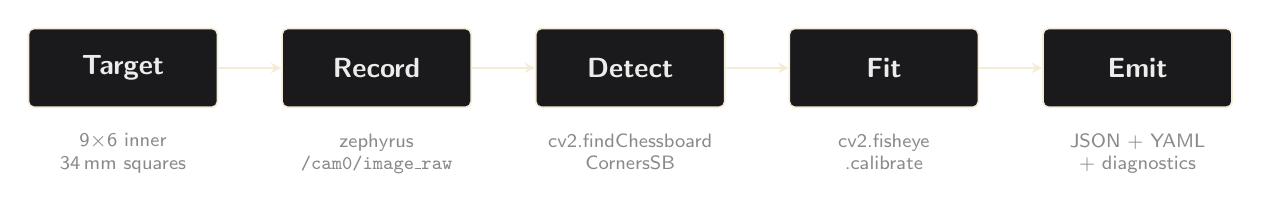
\begin{tikzpicture}[
  font=\sffamily,
  stage/.style={
    draw=ethAccent, line width=0.6pt,
    fill=ethSurface,
    rounded corners=2pt,
    minimum width=2.4cm, minimum height=1.0cm,
    inner sep=6pt,
    text=ethText,
  },
  caption/.style={
    text=ethMuted, font=\sffamily\scriptsize, align=center,
  },
  arrow/.style={-stealth, draw=ethAccent, line width=0.7pt},
]
  \node[stage] (target) {\textbf{Target}};
  \node[stage, right=8mm of target] (record) {\textbf{Record}};
  \node[stage, right=8mm of record] (detect) {\textbf{Detect}};
  \node[stage, right=8mm of detect] (fit)    {\textbf{Fit}};
  \node[stage, right=8mm of fit] (out)       {\textbf{Emit}};

  \draw[arrow] (target) -- (record);
  \draw[arrow] (record) -- (detect);
  \draw[arrow] (detect) -- (fit);
  \draw[arrow] (fit) -- (out);

  \node[caption, below=2mm of target] {9$\times$6 inner\\34\,mm squares};
  \node[caption, below=2mm of record] {zephyrus\\\texttt{/cam0/image\_raw}};
  \node[caption, below=2mm of detect] {cv2.findChessboard\\CornersSB};
  \node[caption, below=2mm of fit]    {cv2.fisheye\\.calibrate};
  \node[caption, below=2mm of out]    {JSON + YAML\\+ diagnostics};
\end{tikzpicture}
\end{center}

\subsection{Why fisheye, not radtan}

The IMX219 wide-angle module on the racing drone has $\sim$131\textdegree{} HFOV. The standard 5-coefficient plumb\_bob (radtan) model loses fidelity past $\sim$120\textdegree{} because radial distortion stops being well-approximated by an even polynomial in $r$. The Kannala-Brandt \emph{equidistant} model parameterises distortion in $\theta$ (the angle from the optical axis) and stays accurate well past 180\textdegree{}.

For drone racing, the relevant detections (gates, ArUco markers) frequently appear at the image periphery during turns. That is precisely where the two models diverge. The OpenVINS configurations already bundled in this repo use the equidistant model for fisheye sensors (\texttt{rs\_t265}, \texttt{uzhfpv\_indoor}), so the choice is consistent with the repo's downstream conventions.

\subsection{Why OpenCV instead of Kalibr}

Kalibr is the canonical tool when joint camera-IMU calibration ($T_{cam,imu}$, time offsets) is needed. For pure intrinsics on a single sensor the OpenCV \texttt{cv2.fisheye} module produces the same Kannala-Brandt parameters with a $\sim$80-line script, no Docker image, and no ROS 1 dependency. The TII reference numbers (the \texttt{calib\_a-trackRATM.json} cited in the issue) were themselves produced by \texttt{cv2.calibrateCamera} based on the schema. Kalibr remains the right tool for the IMU-fusion stage.

\clearpage

% ----------------------------------------------------------------------
% HARDWARE & TARGET
% ----------------------------------------------------------------------
\section{Hardware \& Target}

\subsection{Camera}

\begin{center}
\renewcommand{\arraystretch}{1.25}
\begin{tabular}{@{}>{\sffamily\color{ethMuted}}l l@{}}
\toprule
Sensor                & Sony IMX219 (8 MP CMOS, RAW10, 2$\times$2 binned)\\
Lens                  & Wide-angle variant ($\sim$131\textdegree{} measured HFOV)\\
Host                  & NVIDIA Jetson Orin NX, JetPack 6 (\texttt{aero@zephyrus})\\
Capture pipeline      & \texttt{nvarguscamerasrc} (libargus) $\rightarrow$ \texttt{nvvidconv} $\rightarrow$ gscam2\\
Sensor mode           & 4 — 1280$\times$720, 60 fps stock (no driver mod)\\
Topic                 & \texttt{/cam0/image\_raw} (rgb8)\\
ISP tuning            & exposure 1--5 ms, gain 1--8 (short to limit motion blur)\\
\bottomrule
\end{tabular}
\end{center}

The 90 Hz device-tree mod documented in \texttt{docs/docs/drone-setup/imx219\_90hz\_tuning.md} is \emph{not} required for this calibration; sensor mode 4 publishes at 60 fps on the stock driver and that is what the issue specifies.

\subsection{Calibration target}

\begin{center}
\begin{minipage}[t]{0.55\textwidth}
\renewcommand{\arraystretch}{1.25}
\begin{tabular}{@{}>{\sffamily\color{ethMuted}}l p{0.58\linewidth}@{}}
\toprule
Pattern         & Asymmetric checkerboard\\
Inner corners   & 9 $\times$ 6\\
Squares         & 10 $\times$ 7\\
Square (nominal)  & 35 mm\\
Square (measured) & 34 mm \emph{(97\,\% scale)}\\
Page            & A3 landscape (420\,$\times$\,297 mm)\\
Mounting        & Black tape on white margins, on foam-board\\
Physical board  & Held by Dimetri --- ask before printing your own\\
\bottomrule
\end{tabular}\\[10pt]
\textcolor{ethMuted}{\footnotesize Generator script:}\\
\texttt{\footnotesize scripts/calibration/}\\
\texttt{\footnotesize \quad generate\_checkerboard.py}\\[4pt]
\textcolor{ethMuted}{\footnotesize Generated PDF (ships with the repo):}\\
\texttt{\footnotesize camera\_calibration/}\\
\texttt{\footnotesize \quad checkerboard\_9x6\_35mm\_a3.pdf}
\end{minipage}%
\hspace{0.02\textwidth}%
\begin{minipage}[t]{0.40\textwidth}
\vspace{-2pt}
\begin{tcolorbox}[
  enhanced, colback=ethSurface, colframe=ethRule, boxrule=0.4pt,
  arc=2pt, outer arc=2pt,
  left=4pt, right=4pt, top=4pt, bottom=4pt,
]
\centering
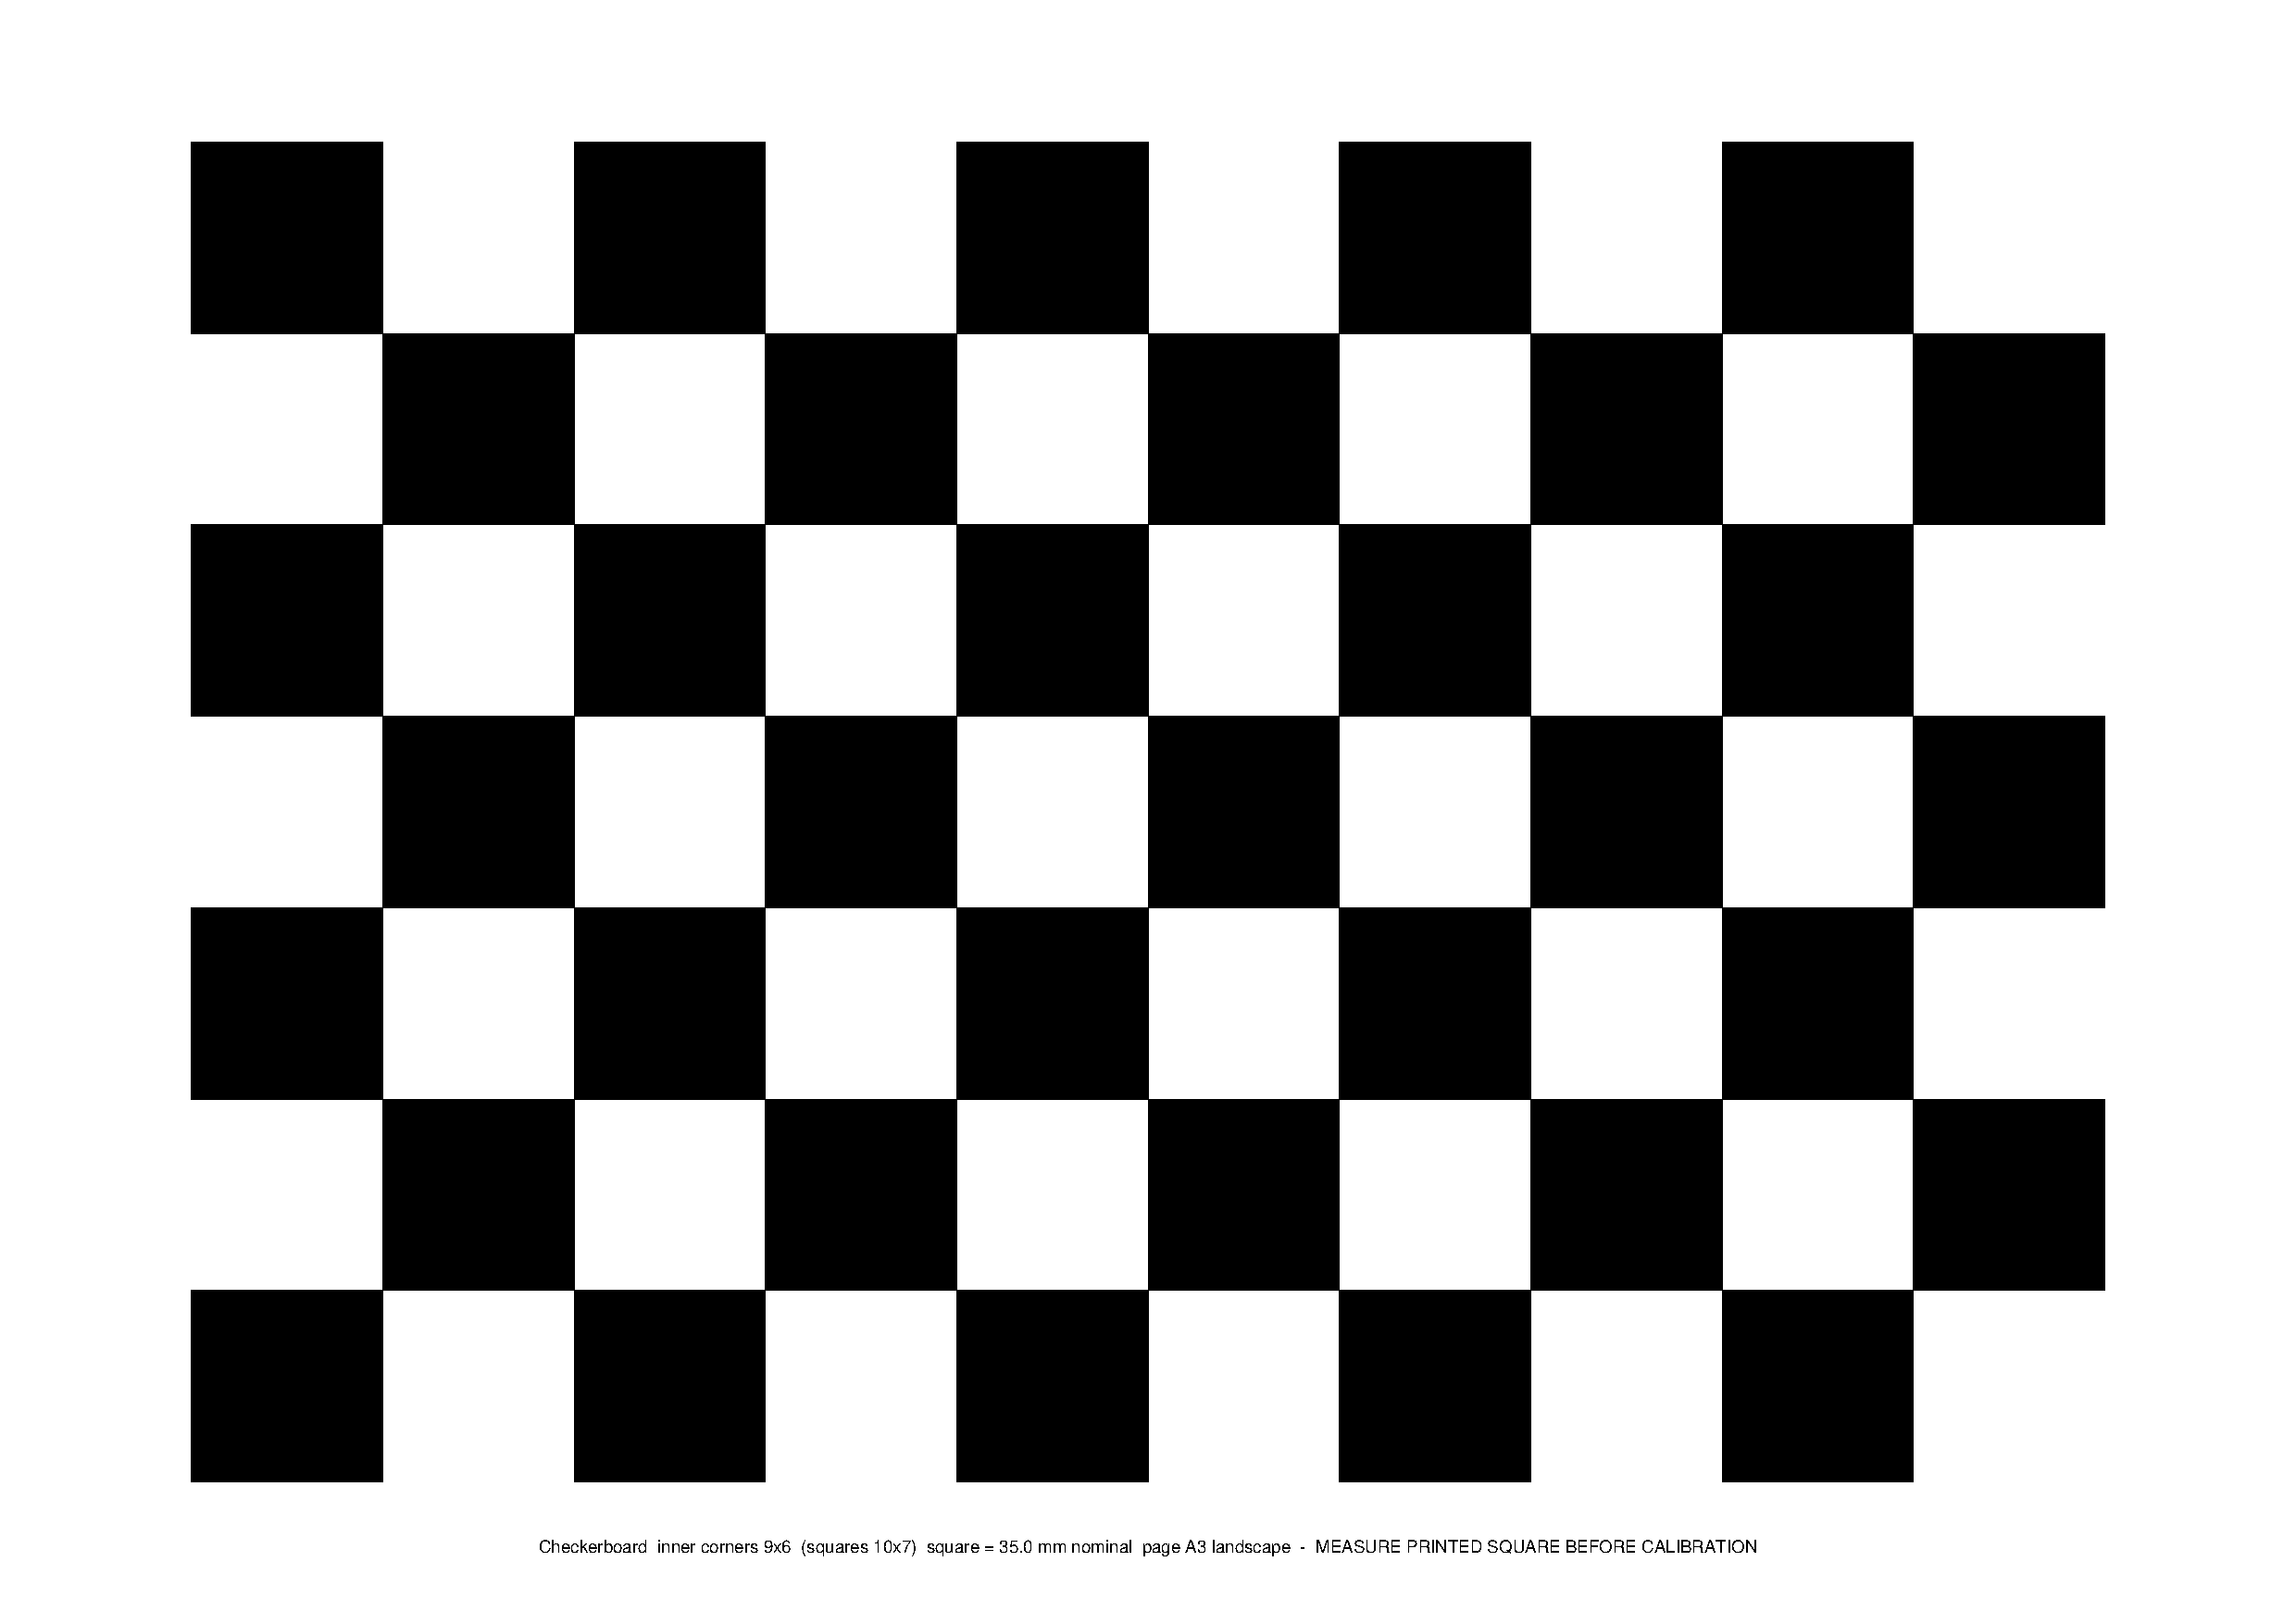
\includegraphics[width=\linewidth, page=1, trim=20pt 100pt 20pt 20pt, clip]{assets/checkerboard_thumbnail.pdf}
\end{tcolorbox}
\textcolor{ethMuted}{\footnotesize\centering The printable target. Squares are checked individually after printing to absorb printer scale variance.}
\end{minipage}
\end{center}

\subsection{Asymmetric pattern: why 9$\times$6 and not 8$\times$8}

\texttt{cv2.findChessboardCornersSB} requires the inner-corner count to be \emph{asymmetric} ($N \neq M$) so that the four-fold rotational ambiguity collapses to a single orientation. 9$\times$6 is the standard ROS Industrial / OpenVINS convention. The detector also requires that \emph{all} inner corners are visible in every accepted frame — partial-board views are silently dropped. \textbf{The physical board for this calibration is held by Dimetri}; ask him before reprinting (the measured 34\,mm square size is specific to that print).

\clearpage

% ----------------------------------------------------------------------
% RECORDING PROCEDURE
% ----------------------------------------------------------------------
\section{Recording Procedure}

The recording script (\texttt{scripts/calibration/record\_bag.sh}) launches the camera node and \texttt{ros2 bag record} in a single foreground session, with SIGINT propagated to the camera's process group on exit.

\begin{codebox}
\$ cd /home/aero/proj/ETHRC-Drone-Racing\\
\$ source install/setup.bash\\
\$ ./scripts/calibration/record\_bag.sh
\end{codebox}

The 90-second waving routine targets \emph{nine specific poses} chosen to exercise the full image plane and a range of incidence angles:

\vspace{4pt}
\begin{center}
\renewcommand{\arraystretch}{1.3}
\sffamily\small
\begin{tabular}{@{}>{\color{ethMuted}}c l l@{}}
\toprule
\# & \color{ethAccentBold}\textbf{Pose} & \color{ethAccentBold}\textbf{Purpose} \\
\midrule
1 & Centre, far ($\sim$70 cm)        & Baseline focal-length signal\\
2 & Centre, close ($\sim$30 cm)      & Multi-distance disambiguation\\
3 & Top-left of frame                & Edge $k_1, k_2$ excitation\\
4 & Top-right of frame               & Edge $k_1, k_2$ excitation\\
5 & Bottom-left of frame             & Edge $k_1, k_2$ excitation\\
6 & Bottom-right of frame            & Edge $k_1, k_2$ excitation\\
7 & Tilt forward $\sim$30\textdegree{} & Pose-rotation conditioning\\
8 & Tilt sideways $\sim$30\textdegree{}& Pose-rotation conditioning\\
9 & Slow diagonal sweep              & Mass coverage across the FOV\\
\bottomrule
\end{tabular}
\end{center}

\vspace{6pt}

\subsection{Live camera preview (essential for placement)}

Moving a calibration target blindly is error-prone, and waiting until after recording to discover the board never reached the corners wastes the whole session. A live MJPEG stream solves this. Two options:

\textbf{Option A --- web\_video\_server (recommended).} Browser-based, no extra software on the laptop, $\sim$150--300 ms latency. One-time install on zephyrus:
\begin{codebox}
\$ sudo apt install -y ros-humble-web-video-server
\end{codebox}
Then in a separate zephyrus terminal (the camera must already be publishing in another terminal --- launching the camera and recording happens elsewhere):
\begin{codebox}
\$ cd /home/aero/proj/ETHRC-Drone-Racing\\
\$ source /opt/ros/humble/setup.bash\\
\$ source install/setup.bash\\
\$ ros2 run web\_video\_server web\_video\_server \textbackslash{}\\
\quad   --ros-args -p port:=8080
\end{codebox}
Find the IP with \texttt{hostname -I} on zephyrus (first listed entry is usually the one your laptop reaches), then open in any browser:
\begin{codebox}
http://<zephyrus-ip>:8080/stream\\
\quad ?topic=/cam0/image\_raw\&type=mjpeg\&quality=70
\end{codebox}
For our hardware the IP is \texttt{192.168.0.77}.

\textbf{Option B --- X11 forwarding.} No install at all, but slower over a typical Wi-Fi link (5--10 fps). On the laptop:
\begin{codebox}
\$ ssh -Y aero@zephyrus\\
\$ cd /home/aero/proj/ETHRC-Drone-Racing \&\& source install/setup.bash\\
\$ ros2 run rqt\_image\_view rqt\_image\_view /cam0/image\_raw
\end{codebox}
Mac users need XQuartz (\texttt{brew install --cask xquartz}, then log out and in).

\subsection{Bag size and on-host processing}

A 90-second 1280$\times$720 60 fps bag at \texttt{rgb8} encoding lands at $\sim$5 GB after rosbag2's chunking. The bag therefore stays on zephyrus: the OpenCV processing script runs there directly via \texttt{uv}, and only the resulting JSON, YAML and PNG outputs ($<$1 MB total) are scp'd back to the laptop. The slow link is removed from the loop entirely.

\subsection{Verifying the camera before recording}

Before pressing record, confirm the camera publishes by opening the preview URL above. The recording script also performs a one-shot health check internally:
\begin{codebox}
{[}INFO{]} launching imx219\_argus\_camera at 1280x720 @ 60 fps\\
{[}INFO{]} /cam0/image\_raw is live\\
{[}INFO{]} recording to bags/imx219\_calib\_<TIMESTAMP>
\end{codebox}
If the second line reports \texttt{[ERROR] /cam0/image\_raw not publishing} the script aborts before any bag is created. Common causes: the workspace is not sourced (re-run both \texttt{source} lines), \texttt{gscam2} is not installed, or another process already holds the CSI sensor (\texttt{ps aux $|$ grep argus} and kill the offender).

\clearpage

% ----------------------------------------------------------------------
% RESULTS
% ----------------------------------------------------------------------
\section{Results}

\subsection{Final intrinsics (Kannala-Brandt equidistant)}

\begin{center}
\begin{tcolorbox}[
  enhanced, colback=ethSurface, colframe=ethRule, boxrule=0.4pt,
  arc=2pt, outer arc=2pt,
  width=\linewidth,
  left=14pt, right=14pt, top=10pt, bottom=10pt,
]
\centering
\sffamily\small
\renewcommand{\arraystretch}{1.4}
\begin{tabular}{@{}>{\color{ethMuted}}l >{\ttfamily\color{ethText}}r@{}}
$f_x$ & 559.381784\\
$f_y$ & 559.454491\\
$c_x$ & 637.688520\\
$c_y$ & 352.823295\\
$k_1$ &  0.067028631\\
$k_2$ & -0.028541814\\
$k_3$ & -0.018213246\\
$k_4$ &  0.058724862\\
\end{tabular}
\\[8pt]
\textcolor{ethMuted}{\footnotesize image size $1280 \times 720$  \quad{}  framerate 60 fps  \quad{}  RMS = 0.6604 px}
\end{tcolorbox}
\end{center}

\subsection{Diagnostics}

\begin{center}
\begin{minipage}[t]{0.46\textwidth}
\centering
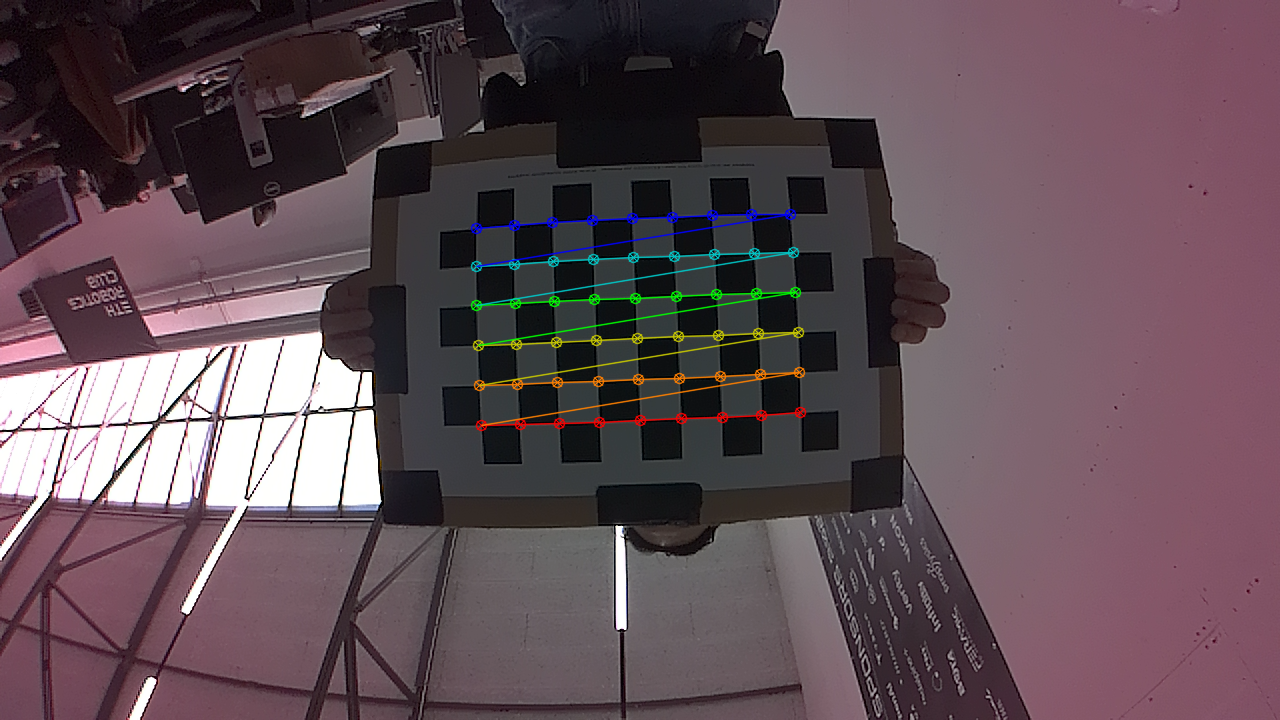
\includegraphics[width=\linewidth]{assets/sample_detection.png}\\[4pt]
\textcolor{ethMuted}{\footnotesize\textbf{Sample detection.} 9$\times$6 inner corners overlaid on a representative frame. The board is held by white margins; the camera is mounted upside-down on the drone (the room ceiling is at the bottom of the image). Image orientation is irrelevant to the intrinsics fit but worth flagging for downstream consumers.}
\end{minipage}%
\hspace{0.04\textwidth}%
\begin{minipage}[t]{0.46\textwidth}
\centering
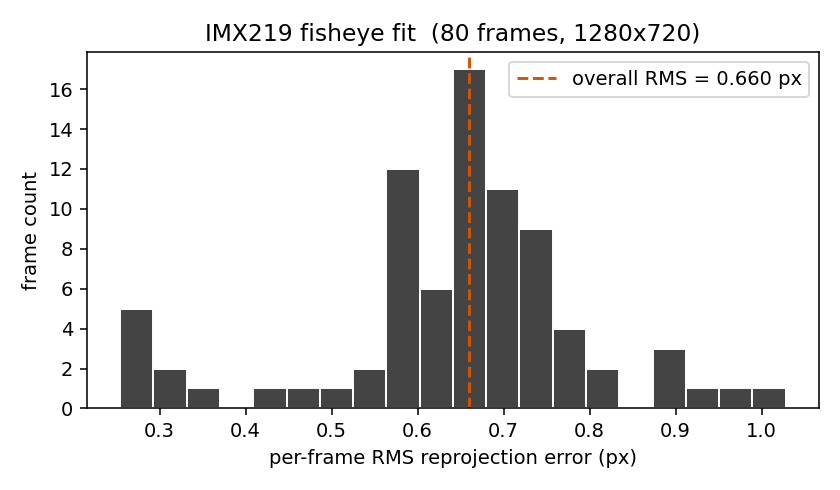
\includegraphics[width=\linewidth]{assets/reprojection_error_hist.png}\\[4pt]
\textcolor{ethMuted}{\footnotesize\textbf{Per-frame reprojection error.} The distribution is unimodal around the overall RMS with a small tail of outliers near 1.0 px. No frames were excluded from the fit; the spread is consistent with handheld waving at $\sim$1 board-width per second.}
\end{minipage}
\end{center}

\subsection{Field-of-view derivation}

The pinhole-projection HFOV from $f_x$ at the chosen resolution:
\[
\mathrm{HFOV} = 2 \cdot \arctan\!\left( \frac{W/2}{f_x} \right)
              = 2 \cdot \arctan\!\left( \frac{640}{559.38} \right)
              \approx 131^{\circ}
\]
The diagonal FOV (using $r_{\mathrm{corner}} = \tfrac{1}{2}\sqrt{W^2+H^2}$ in the \emph{equidistant} formulation $\theta = r/f$) is $\sim$150\textdegree{}. This places the lens firmly in the wide-angle class but well short of the 160--180\textdegree{} extreme fisheye regime sometimes assumed for IMX219 modules.

\subsection{Why radtan and fisheye agree on this bag}

The two fits returned RMS values within 0.01 px of each other (radtan 0.653, fisheye 0.660). For a $\sim$131\textdegree{} HFOV lens the two models genuinely differ in distortion magnitude only at the very corners of the image, and only when the calibration target is held \emph{at} those corners with the board surface non-parallel to the image plane. The current bag has good corner placement but moderate tilt; both models therefore explain the observed corner positions equivalently. This is a recording-coverage artefact, not a model-selection failure --- the fisheye model is still the right one to deploy because at \emph{inference} time gates and markers will appear at the corners with arbitrary geometry.

\subsection{Caveats and known issues}

\begin{itemize}[leftmargin=18pt, itemsep=4pt]
\item \textbf{Image orientation.} The mounted camera is rotated 180\textdegree{}. Downstream consumers should either rotate in the GStreamer pipeline (\texttt{flip-method=2} on \texttt{nvvidconv}) or via an \texttt{image\_rotate\_node}. Intrinsics are unchanged.
\item \textbf{Edge coverage.} A future re-record with the board pressed harder into the very corners (and rotated $\pm$45\textdegree{} there) would tighten the fisheye-vs-radtan separation and is the obvious next experiment if the racing-gate detector shows edge-pixel residuals.
\item \textbf{No IMU coupling.} This calibration is intrinsics-only. The OpenVINS pipeline additionally needs $T_{cam,imu}$ and time offsets, which require a Kalibr camera-IMU run.
\end{itemize}

\clearpage

% ----------------------------------------------------------------------
% REPRODUCTION
% ----------------------------------------------------------------------
\section{Reproduction}

The full pipeline can be re-executed in $\sim$20 minutes once the target is printed. All artefacts live on the \texttt{feature/imx219-calibration} branch.

\subsection{Prerequisites (one-time, on zephyrus)}

Three apt packages and the \texttt{uv} script runner are needed. The colcon build is required only after a fresh clone or a pull that touches the camera package.

\begin{codebox}
\textcolor{ethMuted}{\# ROS 2 packages (require sudo)}\\
\$ sudo apt update\\
\$ sudo apt install -y ros-humble-gscam ros-humble-web-video-server\\[4pt]
\textcolor{ethMuted}{\# uv (no sudo; installs to \textasciitilde{}/.local/bin)}\\
\$ curl -LsSf https://astral.sh/uv/install.sh | sh\\
\$ export PATH="\$HOME/.local/bin:\$PATH"\\[4pt]
\textcolor{ethMuted}{\# Build the camera package once}\\
\$ cd /home/aero/proj/ETHRC-Drone-Racing\\
\$ source /opt/ros/humble/setup.bash\\
\$ colcon build --packages-select imx219\_argus\_camera --symlink-install\\
\$ source install/setup.bash
\end{codebox}

You also need a printed checkerboard. Either reprint the bundled PDF or regenerate it:
\begin{codebox}
\$ ./scripts/calibration/generate\_checkerboard.py\\
\textcolor{ethMuted}{\# Print the resulting PDF on A3 at 100\,\% scale ("Actual size",}\\
\textcolor{ethMuted}{\# not "Fit to printable area"). Measure one square with a ruler;}\\
\textcolor{ethMuted}{\# you will pass this number to the calibration script.}
\end{codebox}

\subsection{File map}

\begin{center}
\sffamily\footnotesize
\renewcommand{\arraystretch}{1.45}
\begin{tabular}{@{}>{\ttfamily\color{ethText}}p{0.55\linewidth} >{\sffamily\color{ethMuted}}p{0.40\linewidth}@{}}
\toprule
\textsf{\bfseries\color{ethAccentBold}Path} & \textsf{\bfseries\color{ethAccentBold}Purpose}\\
\midrule
camera\_calibration/\newline\hspace*{8pt}imx219\_720p\_60fps\_rms066px.json
  & TII-style intrinsics (\texttt{mtx} + \texttt{dist}) plus an explicit fisheye block.\\
camera\_calibration/\newline\hspace*{8pt}imx219\_720p\_60fps\_rms066px\_kalibr.yaml
  & OpenVINS-compatible Kalibr-style YAML.\\
camera\_calibration/\newline\hspace*{8pt}checkerboard\_9x6\_35mm\_a3.pdf
  & Printable target (regenerable).\\
camera\_calibration/sample\_detection.png
  & Corner-detection overlay sample.\\
camera\_calibration/\newline\hspace*{8pt}reprojection\_error\_hist.png
  & Per-frame RMS distribution plot.\\
src/perception/imx219\_argus\_camera/\newline\hspace*{8pt}config/imx219\_720p\_60fps\_rms066px\_kalibr.yaml
  & Same YAML, alongside the camera ROS package.\\
src/perception/imx219\_argus\_camera/\newline\hspace*{8pt}config/camera\_params.yaml
  & Placeholder values replaced with calibrated equidistant model.\\
scripts/calibration/generate\_checkerboard.py
  & Re-renders the target PDF (uv inline deps).\\
scripts/calibration/record\_bag.sh
  & Drives \texttt{ros2 bag record} on zephyrus.\\
scripts/calibration/calibrate\_imx219.py
  & Bag\,$\rightarrow$\,intrinsics; uv inline deps. Output filenames carry the achieved RMS.\\
\bottomrule
\end{tabular}
\end{center}

\subsection{End-to-end commands}
\nopagebreak

The five steps below assume the prerequisites are satisfied and the printed target is on a flat board. Lines ending in \texttt{\textbackslash{}} are bash continuations.
\nopagebreak

\begin{codebox}
\textcolor{ethMuted}{\# 1. SSH in and refresh the branch.}\\
\$ ssh aero@zephyrus\\
\$ cd /home/aero/proj/ETHRC-Drone-Racing\\
\$ git checkout feature/imx219-calibration \&\& git pull --ff-only\\
\$ source install/setup.bash\\[6pt]
\textcolor{ethMuted}{\# 2. (Optional but strongly recommended) start the live preview}\\
\textcolor{ethMuted}{\#    in a SECOND zephyrus terminal so you can see what you record.}\\
\$ ros2 run web\_video\_server web\_video\_server \textbackslash{}\\
\quad   --ros-args -p port:=8080\\
\textcolor{ethMuted}{\#    Then on the laptop, open in a browser:}\\
\textcolor{ethMuted}{\#    http://<zephyrus-ip>:8080/stream?topic=/cam0/image\_raw\&type=mjpeg}\\[6pt]
\textcolor{ethMuted}{\# 3. Record a 60--120 s waving session (back in the FIRST terminal).}\\
\$ ./scripts/calibration/record\_bag.sh\\
\textcolor{ethMuted}{\#    Wave the printed board through the 9 poses listed in section 3,}\\
\textcolor{ethMuted}{\#    watching the preview to confirm coverage. CTRL+C to stop.}\\[6pt]
\textcolor{ethMuted}{\# 4. Process the bag on zephyrus (no need to transfer the GB-scale bag).}\\
\textcolor{ethMuted}{\#    --square-size-mm = MEASURED size of one printed square.}\\
\$ ./scripts/calibration/calibrate\_imx219.py \textbackslash{}\\
\quad   --bag bags/imx219\_calib\_<TIMESTAMP> \textbackslash{}\\
\quad   --square-size-mm 34.0\\[6pt]
\textcolor{ethMuted}{\# 5. From your LAPTOP, pull the small JSON+YAML+PNG outputs back.}\\
\textcolor{ethMuted}{\#    Variable + escaped \textbackslash{}* keeps the glob unexpanded locally so}\\
\textcolor{ethMuted}{\#    sshd expands it on zephyrus.}\\
\$ cd <local-clone-of-the-repo>\\
\$ ZEPH=aero@zephyrus:proj/ETHRC-Drone-Racing/camera\_calibration\\
\$ scp "\$ZEPH"/imx219\_720p\_60fps\textbackslash{}* camera\_calibration/
\end{codebox}

\subsection{Validation}

A successful run prints:
\begin{itemize}[leftmargin=18pt, itemsep=2pt]
\item \texttt{{[}INFO{]} locked pattern orientation = (9, 6) (as configured)} --- auto-detected board orientation.
\item \texttt{{[}INFO{]} N frames detected so far ...} --- non-zero, ideally 50--80 by completion.
\item \texttt{{[}INFO{]} fisheye RMS = 0.X px} --- should be $<$1.0; ideally $<$0.7.
\item \texttt{{[}OK{]} wrote camera\_calibration/imx219\_720p\_60fps\_rmsXXXpx.json} --- with the achieved RMS auto-encoded in the filename.
\item Four output files in total under \texttt{camera\_calibration/}: JSON, Kalibr YAML, sample-detection PNG, error-histogram PNG.
\end{itemize}

If RMS exceeds 1 px, re-record with the board pushed harder into the four image corners (where most of the distortion signal lives) and held still longer at each pose.

\subsection{Future work}

\begin{enumerate}[leftmargin=18pt, itemsep=4pt]
\item \textbf{Camera-IMU joint calibration.} Re-record with the IMU also publishing, and process with Kalibr (\texttt{kalibr\_calibrate\_imu\_camera}) to recover $T_{cam,imu}$ and time offsets. Required for OpenVINS / VINS-Fusion deployment.
\item \textbf{Stereo or multi-camera.} If a second IMX219 is added, re-use the same recording script with \texttt{/cam1} appended; the script generalises trivially.
\item \textbf{Edge-rich re-record.} Push the board harder into the four corners with steep tilts to tighten the fisheye-vs-radtan separation.
\item \textbf{Image flip in pipeline.} Add \texttt{flip-method=2} to the \texttt{nvvidconv} step in \texttt{gscam\_imx219.yaml} so consumers receive a right-side-up frame.
\end{enumerate}

\vspace{20pt}

\begin{pillar}
\textbf{One sentence.}  This document records a single intrinsics calibration of one specific physical lens at one resolution and frame-rate; if any of those three change (lens swap, mode change, sensor swap), the calibration must be re-run.
\end{pillar}

\vfill
\noindent
\textcolor{ethMuted}{\sffamily\footnotesize
\textcolor{ethRule}{\rule{\linewidth}{0.4pt}}\\[6pt]
ETH ROBOTICS CLUB  \quad\textbar\quad  Drone Racing  \quad\textbar\quad  v1.0  \quad\textbar\quad  All rights reserved}

\end{document}
